\section{Problems}

Here is a link to my code: \url{https://github.com/filipmellgren/QMM/tree/main/ps4}.

\begin{questions}
\question{Life cycle questions}
\begin{solution}
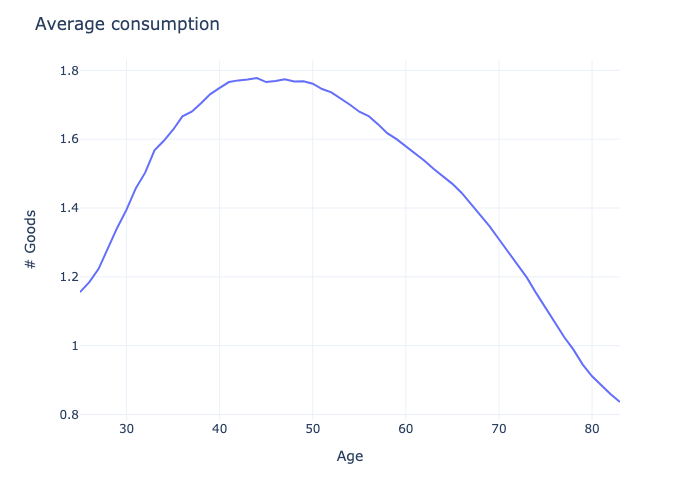
\includegraphics[scale=0.5]{figures/mean_cons.png}
\includegraphics[scale=0.5]{figures/mean_inc.png}
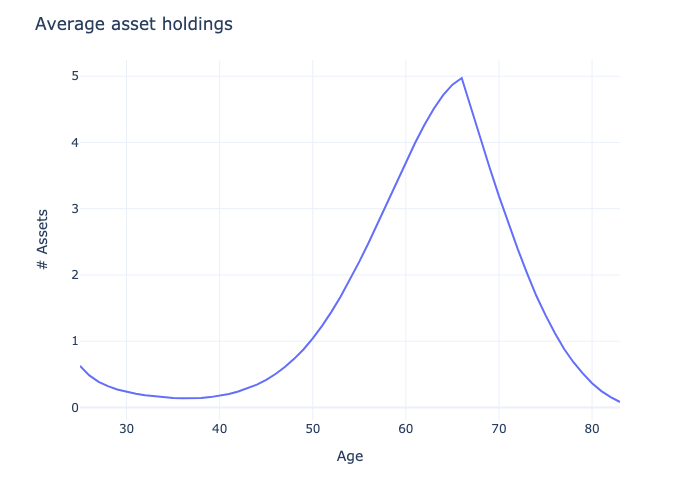
\includegraphics[scale=0.5]{figures/mean_assets.png}
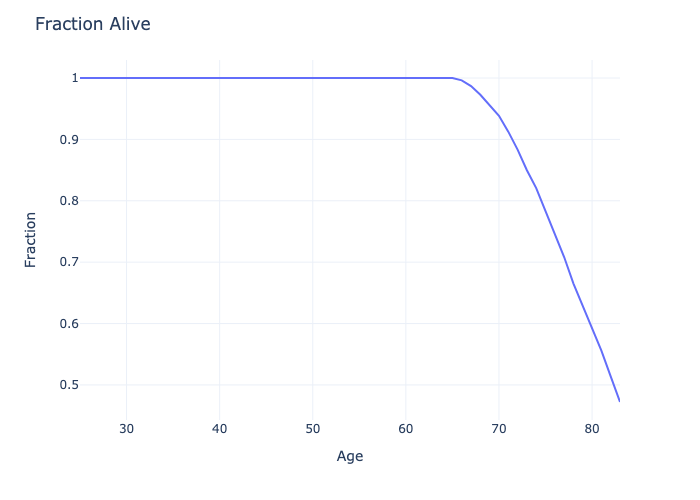
\includegraphics[scale=0.5]{figures/fraction_alive.png}

I don't understand what is meant in 1.3.2, so I skip that.

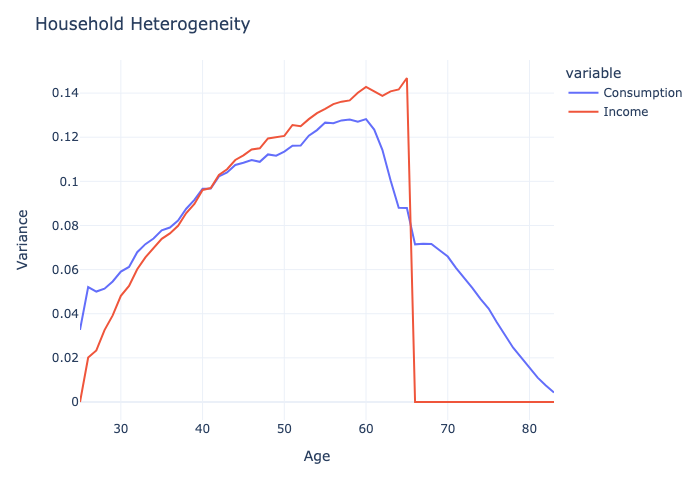
\includegraphics[scale=0.5]{figures/hh_heterogeneity.png}
In the initial periods, there is more consumption heterogeneity between households than differences in income. 

\end{solution}

\question{Insurance questions}
\begin{solution}
A higher rho (i.e. persistence in income shocks), is associated with a lower ratio of $\frac{\operatorname{cov}\left(\Delta c_{i t}, n_{i t}\right)}{\operatorname{var}\left(n_{i t}\right)}$, which is a measure of insurance. A high positive value is no insurance, and 0 means the change in consumption is uncorrelated with the shocks, i.e. perfect insurance. 

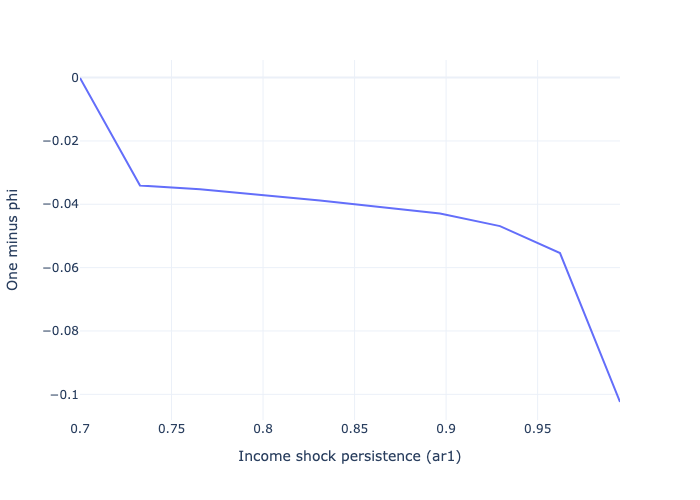
\includegraphics[scale=0.5]{figures/insurance_question.png}

\end{solution}
\end{questions}


